\section{Code Generation}
\label{sec:codegen}

\subsection{Overview}

Code generation~\cite{llvm:backend} is the task to generate the target specific machine code from the LLVM IR.
The code generation is one of the more complicated processes in the LLVM, it is performed
over several passes(steps) in which we will go into in the next few sections. Each pass "lowers"
the intermediate representation a little more towards the final machine code. During this process
the code is optimized for the target platform, unsupported operations and data types are replaced,
registers are allocated and so on. LLVM backends which do the actual code generations, are written
with the help of the \textbf{target-independent code generator} framework~\cite{llvm:targetindependent}. 
This work described the overall functionality and mechanisms of this LLVM framework.

The target-independent code generator framework uses the following phases:
\begin{enumerate}
  \item Instruction Selection
  \item Scheduling and Formation
  \item SSA-based Machine Code Optimizations
  \item Register Allocation
  \item Final Optimizations
  \item Code Emission
\end{enumerate}
The \textit{Instruction Selection} is itself subdivided in even more passes, this will be discussed 
in section~\ref{subsec:instruction_selection}.

Let's consider the C code version of the LLVM IR example which was shown in section~\ref{subsec:llvm_ir}.
\begin{lstlisting}[language=C]
  int foo(int aa, int bb, int cc) {
    int sum = aa + bb;
    return sum / cc;
  }
\end{lstlisting}
This example of a simple C function is compiled into the LLVM IR by using the clang frontend: 
\lstinline[language=bash]{clang -cc1 foo.c -emit-llvm}. 
The resulting IR code is still very similar, and you can easily recognize the original program code.
\begin{lstlisting}[language=LLVM,label={lst:llvm_simple}]
define i32 @foo(i32 %aa, i32 %bb, i32 %cc) {
  entry:
    %add = add nsw i32 %aa, %bb
    %div = sdiv i32 %add, %cc
    ret i32 %div
}
\end{lstlisting}
This IR representation is the basis of LLVM's code generator. The actual transformations of the code generator
will takes place on another form of the IR code, an \textbf{directed acyclic graph}.

\subsection{Instruction Selection}
\label{subsec:instruction_selection}

\subsubsection{Directed Acyclic Graph}

The directed acyclic graph (DAG) represents the program as nodes and connections (essentially a tree),
which each represent an operation, variables or results. The reason for using a DAG is that
it is easy to represent a program flow in this way and then perform transformations directly on the DAG.
A DAG can contain generally the following objects:
\begin{enumerate}
  \item Leaf nodes represent identifiers, names or constants.
  \item Interior nodes can represent operators.
  \item Interior nodes also represent results of expressions or identifiers of locations where values are to be stored.
\end{enumerate}

A simple DAG corresponding to the previously~\ref{lst:llvm_simple} shown C function:
\begin{figure}
    \centering
    \begin{subfigure}[b]{0.45\textwidth}
        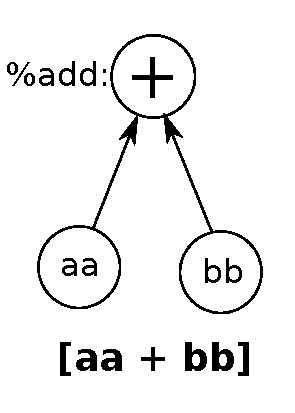
\includegraphics[width=.5\textwidth]{../slides/pictures/dag_step_1}
        \caption{The first add operation}
        \label{fig:dag_fmadd}
    \end{subfigure}
    ~ %add desired spacing between images, e. g. ~, \quad, \qquad, \hfill etc. 
      %(or a blank line to force the subfigure onto a new line)
    \begin{subfigure}[b]{0.45\textwidth}
        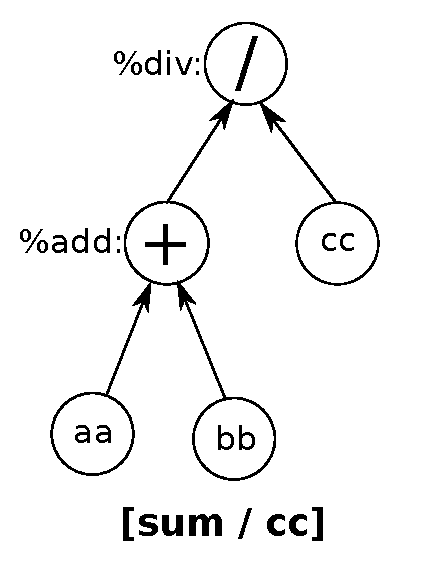
\includegraphics[width=.65\textwidth]{../slides/pictures/dag_step_2}
        \caption{Division using the add result}
    \end{subfigure}
\end{figure}


\subsubsection{DAG Construction}

In LLVM the actual DAG looks a little more complicated. The first pass of the Instruction Selection process is to build 
the \textbf{SelectionDAG} from the LLVM IR. The code generator framework does this in a target independent way through the 
\lstinline[language=c++]{SelectionDAGBuilder} class. This builder class uses target specific callbacks provided by the code generation
backend (within an instance \lstinline[language=c++]{TargetLowering}) to include as much target specific information as possible
with each node of the tree. The nodes in the SelectionDAG are instances of the \lstinline[language=c++]{SDNode} class, whose 
primary payload is the node type (opcode) of the operation it represents. 
LLVM defines a series of opcodes (defined in ISDOpcodes.h), which correspond to every operation  
supported in the LLVM IR. Every node defines one or more return values, which can be used by other nodes
connected with it. For example a modulo operation is maybe expressed as a division which also provides the remainder.
The edges of a node are defined as a pair of the target SDNode and an index identifying the return value which should be used.
Every return value provided by a SDNode operation is has an associated data type (integer, floating-point, vector, \dots).

The SelectionDAG enables the compiler backend to use techniques like pattern matching selectors, to choose instructions and 
operators to transform. As we will see in later examples, a backend developer can specify complex patterns of operations
(e.g.\ combination of multiplication and addition operations) and replace them with other operations (which are optimized,
actually supported on the platform etc.). 
One more concept which neeeds to be introduced in this section, is the concept of legal and illegal DAGs. Because the SelectionDAG
was generated without many considerations for target-dependent particularities, there may be operations or datatypes which are not
supported by the target. All processing passes during the instruction selection will gradually transform the SelectionDAG
into a legal form and optimize the used operations. 

\subsubsection{Legalize SelectionDAG}
\label{subsec:legalize}

The next step in the instruction seclection phase is to make sure all \textit{data-types} and \textit{operations} used in the SelectionDAG 
are supported by the target architecture. For example a target might require that all single floating point values 
are promoted to doubles or that bytes/shorts are handled as 32bit integers.
The following operations have to be applied until all types in the SelectionDAG are \textit{legal}:
\begin{itemize}
  \item Promoting: Small types are transformed into larger types.
  \item Expanding: Large integer types are broken up into smaller ones.
\end{itemize}

For example let's look at the loading of a 1-bit (boolean) value on the SPARC architecture. The value for this type would have to 
be sign extended (padded with zeros or ones) to fit into CPU registers. The code generation framework promoted the type automatically
if the developer specifies it in the configuration with this command:
\begin{lstlisting}[language=C++]
setLoadExtAction(ISD::SEXTLOAD, MVT::i1, Promote);
\end{lstlisting}

Other types which are not be supported, might need to be broken down into smaller types. The same applies to operations, on
SPARC the signus and cosinus operations are not supported on 32 bit floating point numbers.
This means they will have to be replaced with a series of instructions, which perform equivalent operations. The developer of
a new code generation backend can indicate this with: 
\begin{lstlisting}[language=C++]
setOperationAction(ISD::FSIN, MVT::f32, Expand);
setOperationAction(ISD::FCOS, MVT::f32, Expand);
\end{lstlisting}
The target-independent code generation algorithm knows how to replace these commands automatically. 
By default all operations are assumed to be legal, this way the code generator can perform the
transformation using only supported operations.
This is an example of how target-specific information is abstracted away from the framework. In some instances custom handling
is required, it is possible to specify custom functions to handle certain operations.  

\subsubsection{Optimize SelectionDAG Pass: The DAG combiner}

The optimization of the SelectionDAG is performed multiple times.
It is executed three times in total, immediately after the DAG is build and once after each legalization.
First in the beginning on the original DAG to clean op the initial code provided by the frontend.
This allows the optimizer to perform optimizations  which depend on knowledge of the original data types.
Another optimization pass is executed after each "legalization" phase. These clean up 
the potentially messy code generated by these passes and allows them to remain simple.

Once class of optimizations is for example the removal of unnecessarily inserted sign and zero extensions.
Sign extensions is the process of increasing the number of bits used store a number, while keeping the sign (+/-).
This is performed by appending $0$'s or $1$'s digits to the most significant side of the number. For positive numbers
$0$ is added, for negative values (represented as two complement) $1$'s are added.
Sign and zero extensions are required to load values which have a smaller data type than the register they are loaded into.
For example when you have programs using lots of 32-bit integer values (as Java's \textit{int} type for example) 
(JIT) compiling for a 64-bit architecture, many 32-bit values must be sign-extended to 64-bit values 
for integer operations~\cite{Kawahito:2002:ESE:543552.512552}.
The optimizer takes care of removing unnecessary instructions, or replacing slow instructions with faster ones.

\subsubsection{Select Phase Selection}

The SelectionDAG is transformed into another DAG based on nodes of the \lstinline[language=c++]{MachineSDNode} class.
This backend developer specifies patterns to match the legal SelectionDAG nodes to this new target DAG, which contains 
the actual opcodes for the target architecture.
An instance of \lstinline[language=c++]{MachineSDNode} contains all information 
necessary to generate the machine code instructions.

To again look at an example, this code will be converted into an equvivalent DAG:
\begin{lstlisting}[language=LLVM,label={lst:llvm_example}]
  %t1 = fadd float %W, %X
  %t2 = fmul float %t1, %Y
  %t3 = fadd float %t2, %Z
\end{lstlisting}

%\begin{wrapfigure}[15]{R}{0.2\textwidth}
%    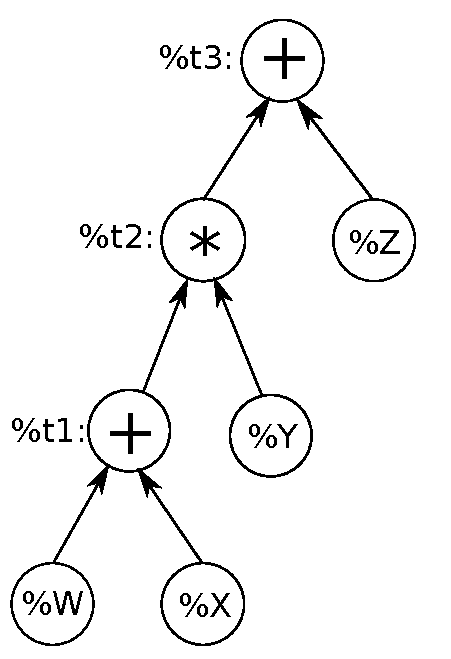
\includegraphics[width=0.19\textwidth]{../slides/pictures/dag_mul_add}
%  \caption{SelectionDAG visualization of the LLVM code in~\ref{lst:llvm_example}}
%\end{wrapfigure}

The SelectionDAG for this corresponds to this (using a more compact textual representation):
\begin{lstlisting}
(fadd:f32 (fmul:f32 (fadd:f32 W, X), Y), Z)
\end{lstlisting}
In this code sample, fadd and fmul are simple add and multiply operations. These instructions can be matched
one-to-one to machine instructions. Some archtectures (like PowerPC) support fused-multiple-add (FMA) operations, which 
multiply the first two parameters and add the third ($X * Y + Z$).
by using this the backend developer for PowerPC can specify a pattern, which eleminates one extra fadd instruction:
\begin{lstlisting}
(FMADDS (FADDS W, X), Y, Z)
\end{lstlisting}


\subsection{Scheduling and Formation}

Takes the DAG, which now contains the actual target instructions.
The Scheduler assigns an order to every node which contains an instruction. The scheduling algorithm needs to take 
the constraints of the machine into account, e.g.\:
\begin{itemize}
  \item Optimize order for minimal register pressure, i.e.\ since the number of registers is limited we want 
        to minimize the number of memory loads or stores (\textit{spills} and \textit{reloads}).
  \item Take instruction latencies into account.
\end{itemize}
In the end this pass outputs a list of machine instructions, the DAG is discarded since it is no longer needed.

\subsection{Register Allocation}

All opperations at this point still operate on an unlimited amount of \textit{virtual registers} . 
These need to be mapped to a limited amount of \textit{physical registers}, provided by the CPU.
When the number of physical registers is not big enough, we need to map some 
virtual registers into memory. These virtual registers are called \textit{spilled virtuals}.

\subsection{Prolog/Epilog Code Insertion}

Sometimes functions exit unexpectedly, for example through an exception.
Throwing an exception in a function requires \textit{unwinding}.
Every time a function calls another function, the calling functions registers are written onto the \textit{call stack}
as a \textit{stack frame}. The call stack stores information about the active functions of the program. 
The reason using the stack is to keep track of the point to which each active function must return control to.
When an exception is thrown it is handled in a \textit{catch block} somewhere in a function.
Stack unwinding means to clean up the stack frames of the functions below this function's frame.
For example in C++ all the objects need to be deallocated.

\subsection{Code Emission}

At this point in the code generation process, the representation of the machine instructions is still
equivalent to assembly code. There are still labels used to identify locations in the code, as well
as \textit{directives}. Directives are commands which influence the code emission (For example to place
a string in the object file).
If the compiler is supposed to output an executable file (or an object file) the compiler backend 
needs to implement ah assembler. Calculating adresses for global variables, calculating jump tables and much
more.